\section{Some classic CNN models}\label{sec:CNNs}
In this section, we will use the notation introduced above to 
give a brief description of some classic CNN models.

\subsection{LeNet-5, AlexNet and VGG}
The  LeNet-5 \cite{lecun1998gradient}, AlexNet \cite{krizhevsky2012imagenet} and VGG \cite{simonyan2014very}
can be written as:
	\begin{equation}
	\begin{cases}
	f^{1,0} &= \theta^0(f), \\
	f^{\ell,i} &= \theta^{\ell,i} \circ \sigma (f^{\ell, j-1}), \quad i = 1:\nu_\ell ~\text{and}~ \ell = 1:J,\\
	f^{\ell+1,0} &= R_\ell^{\ell+1}( f^{\ell,m+\ell}).  \\
	\end{cases}
	\end{equation}
	where $R_\ell^{\ell+1}$ can be general pooling operators and $\theta^{\ell,i}$ can be convolution with stride 1, 
	or fully connected operators.  
	Then the CNN model will be defined by
	\begin{equation}\label{eq:cnndefine}
	H_0(f) = f^{L,\nu_\ell}.
	\end{equation}
	In these three classic CNN models, they still need some 
	extra fully connected layers in nonlinear mapping $H_0$ before the logistic regression as it contains 
	a fully connected layer as in \eqref{eq:log_reg}. 
	These fully connected layers are removed in ResNet to be described below.
\subsection{ResNet}
The ResNet \cite{he2016deep} can be written as
	\begin{equation}\label{ori-ResNet}
	\begin{cases}
	f^{1,0} &=R_{\rm max}\circ \sigma \circ \theta^0(f), \\
	f^{\ell,i} &= \sigma \left( f^{\ell, i-1} + \mathcal{F}^{\ell, i} (f^{\ell,i-1}) \right), \quad i = 1:\nu_\ell ~\text{and}~ \ell = 1:J ,\\
	f^{\ell+1,0} &= \sigma \left( R_\ell^{\ell+1} (f^{\ell, \nu_\ell} )+ \mathcal{F}^{\ell, 0} (f^{\ell, \nu_\ell} ) \right), \quad \ell = 1:J-1,\\
	H_0(f) &=  R_{\rm ave}(f^{L,\nu_\ell}). \\
	\end{cases}
	\end{equation}
	Here
	$$
	\mathcal{F}^{\ell,i} (f^{i-1}) = \xi^{i} \circ \sigma \circ \eta^{i} (f^{i-1}).
	$$
	Generally, $\xi^{\ell,i}$ and $\eta^{\ell,i}$ takes the form of \label{eq:conv-1} with zero padding and stride 1,
	except, $\eta^{\ell,0}$  is taken as convolution with stride 2 with the same output dimension of $R_\ell^{\ell+1}$.
	
\subsection{iResNet} 
	The iResNet\cite{he2016identity} can be written as:
	\begin{equation}\label{eq:iResNet1}
	\begin{cases}
	f^{1,0} &=R_{\rm max}\circ \sigma \circ \theta^0(f), \\
	f^{\ell,i} &= f^{\ell, i-1} + \mathcal{F}^{\ell, i} (f^{\ell,i-1}), \quad i = 1:\nu_\ell ~\text{and}~ \ell = 1:J ,\\
	f^{\ell+1,0} &=  R_\ell^{\ell+1} (f^{\ell, \nu_\ell} )+ \mathcal{F}^{\ell, 0} (f^{\ell, \nu_\ell} ) , \quad \ell = 1:J-1,\\
	H_0(f) &=  R_{\rm ave}(f^{L,\nu_\ell}). \\
	\end{cases}
	\end{equation}
	where
	$$
	\mathcal{F}^{\ell,i} (f^{\ell,i -1}) = \xi^{\ell,i} \circ \sigma \circ \eta^{\ell,i} \sigma (f^{\ell,i-1}).
	$$
	The only difference between ResNet and iResNet can be viewed as 
	putting a $\sigma$ in different places. 
	The connection of those three models are often shown with next diagrams:
	\begin{figure}[!htb]
		\begin{center}
			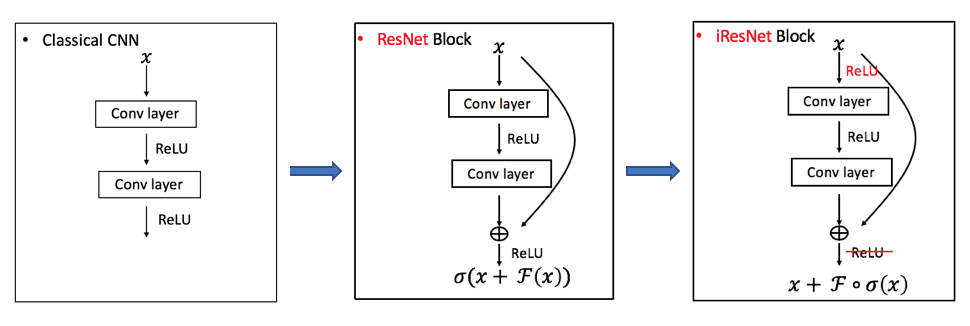
\includegraphics[width=.6\textwidth, height=.13\textheight]{comparison-net} 
		\end{center}
		\caption{Comparison of CNN Structures}
	\end{figure}
	

Without loss of generality, we extract the key 
feedforward steps on the same grid in different CNN models as follows.
\begin{description}
	\item[Classic CNN] 
	\begin{equation}\label{eq:cCNN}
	f^{\ell,i} = \xi^i \circ \sigma (f^{\ell,i-1}) \quad \text{or} \quad f^{\ell,i} = \sigma \circ \xi^{i} (f^{\ell,i-1}) .
	\end{equation}
	\item[ResNet] 
	\begin{equation}\label{eq:ResNet}
	f^{\ell,i} = \sigma( f^{\ell,i-1} + \xi^{\ell,i} \circ \sigma \circ \eta^{\ell,i}(f^{\ell,i-1})).
	\end{equation}
	\item[iResNet]
	\begin{equation}\label{eq:iResNet}
	f^{\ell,i} = f^{\ell,i-1} + \xi^{\ell,i} \circ \sigma \circ \eta^{\ell,i}\circ \sigma(f^{\ell,i-1}).
	\end{equation}
\end{description} 

